\chapter{観測機器}
本章では、観測に使用したX線天文衛星XRISM と検出器 SXI について、また 静止気象衛星 GOES と 検出器 XRS について紹介する。

\section{X線分光撮像衛星 XRISM}

\begin{figure}[H]
	\centering
	\includegraphics[width=0.6\linewidth]{Chapter3/Figures/xrism.png} 
	\caption{XRISM 衛星の外観\cite{xrism_sat_overlook}}
	\label{fig:xrism_sat_overlook}
\end{figure}

X線分光撮像衛星 XRISM (X-Ray Imaging and Spectroscopy Misson)(Tashiro, M. et al., 2022\cite{tashiro_2024})
は「はくちょう」「ぎんが」「てんま」「あすか」「すざく」「ひとみ」に次ぐ日本で 7 番目のX線天文衛星である。
XRISM は 2023 年 9 月 7 日に種子島宇宙センターから打ち上げられた。
図\ref{fig:xrism_sat_overlook} に XRISM の外観を示す。
XRISM はX線マイクロカロリメータとX線望遠鏡から構成される Resolve (Ishisaki, Y. et al., 2022\cite{ishisaki_2022})と、
X線 CCD カメラとX線望遠鏡から構成される Xtend (Mori, K. et al., 2022\cite{mori_2022})の 2 台の検出器を搭載している。
XRISM は Resolve による高い分光性能と、Xtend による広い撮像視野を用いて、
宇宙の高温プラズマにおける物質循環とエネルギー輸送過程と天体の進化の解明を進めること目標にしている。
具体的には以下を目標に掲げている。
\begin{itemize}
	\item 宇宙の構造形成と銀河団の進化
	\item 宇宙の物質循環の歴史
	\item 宇宙のエネルギー輸送と循環
\end{itemize}

\section{XMA}


\begin{figure}[htbp]
	\begin{center}
		\centering
		%\includegraphics[width=0.4\linewidth]{Chapter3/Figures/xrism_xma_xtend_resolve.jpg} 
		\includegraphics[width=0.8\linewidth]{Chapter3/Figures/two_XMA.jpg} 
		\caption{XMA の外観\cite{xrism_pog}。
			左が Xtend-XMA、右が Resolve-XMA である。}
		\label{fig:xma_overlook}
	\end{center}
\end{figure}

\begin{figure}[htbp]
	\begin{center}
		\centering
		\includegraphics[width=0.6\linewidth]{Chapter3/Figures/xrism_xma_xtend_resolve.jpg} 
		\caption{XMA, Xtend, Resolve の配置位置 \cite{xrism_pog}}
		\label{fig:xrism_xma_xtend_resolve}
	\end{center}
\end{figure}


\begin{table}[H]
	\begin{center}
		\centering
		\caption{XMA の性能}
		\label{tab:XMA_basic_param}	
		\begin{tabular}{ll}
			\hline
			\hline
			焦点距離 & 5.6 m\\
			有効開口直径 & 12--35 cm\\
			入射角 & 0.15°--0.57°\\      
			エネルギー範囲 & 0.3--15 keV\\ 
			有効面積 & 約 580 cm\textsuperscript{2} (1.5 keV)\\
			& 約 418 cm\textsuperscript{2} (6.4 keV)\\
			角分解能 (HPD) & 1.5′ (Xtend-XMA)\\
			\hline
		\end{tabular}
	\end{center}
\end{table}


XMA (X-ray Mirror Assembly) は XRISM に搭載されているX線望遠鏡である。図\ref{fig:xma_overlook} に XMA の外観を示す。
XMA は反射鏡のペアを同心円状に 203 枚並べた構造をしており、これらを結合することで焦点距離 5.6~m の一つの望遠鏡としている。
XRISM にはこの XMA が 2 台搭載されており、それぞれが Xtend と Resolve に X線光子を集光するために使用される。
本論文ではそれぞれを Xtend-XMA、Resolve-XMA と呼ぶ。
図\ref{fig:xrism_xma_xtend_resolve}に衛星上での XMA, Xtend, Resolve の配置を示す。
また、表\ref{tab:XMA_basic_param} に XMA の性能を示す。

\subsection{有効面積}

\begin{figure}[H]
	\begin{center}
		\centering
		\includegraphics[width=0.8\linewidth]{Chapter3/Figures/xma_eff.jpg} 
		\caption{Xtend-XMA と Resolve-XMA の有効面積\cite{xrism_pog}。
			左図が liner scacle、右図が log scale 表記である。
			また、図中の黒線が Xtend-XMA、赤線が Resolve-XMA である。}
		\label{fig:xma-eff}
	\end{center}
\end{figure}

有効面積とは光軸方向から見たX線望遠鏡の開口面積に反射鏡の反射率をかけたものであり、
X線を集光する実効的な面積を表す。
図\ref{fig:xma-eff} に Xtend-XMA と Resolve-XMA の有効面積を示す。
この有効面積は地上試験によって得られた有効面積を元に ray-tracing シミュレーションによって計算されている。

\subsection{PSF}
\begin{figure}[H]
	\begin{center}
		\centering
		\includegraphics[width=0.8\linewidth]{Chapter3/Figures/xma_psf_plot.jpg} 
		\caption{Resolve-XMA と Xtend-XMA における PSF\cite{Tamura_K_2022}。
			左図が Resolve-XMA、右図が Xtend-XMA である。}
		\label{fig:xma_psf_image}
	\end{center}
\end{figure}

PSF (point spread function) とは、点源を入射し撮像した時にどのように像が広がるかを表す関数である。
図\ref{fig:xma_psf_image} に Resolve-XMA と Xtend-XMA の PSF を示す。
PSF は点源の位置に鋭いピークを持ち、そこから離れるにつれて急速に値が小さくなっていく半径依存性を持った関数となる。
また、PSF はエネルギー依存性を持ち、エネルギーが大きくなるにつれてより視野中心から光子が広がる特徴を持つ。
%図\ref{fig:xma_psf_image} に on-axis における 6 つの異なるエネルギーのX線を照射した時の Xtend-XMA と Resolve-XMA における PSF を示す。

%\begin{figure}[H]
%	\begin{center}
	%		\centering
	%		\includegraphics[width=0.8\linewidth]{Chapter3/Figures/xma_psf_image.jpg} 
	%		\caption{Resolve-XMA と Xtend-XMA における PSF の構造図 \cite{Tamura_K_2022}。
		%		上図が Resolve-XMA、下図が Xtend-XMA。
		%		入射したX線のエネルギーはそれぞれ 1.49, 4.50, 6.40, 8.05, 9.44, 11.07~keV である。}
	%		\label{fig:xma_psf_image}
	%	\end{center}
%\end{figure}
\newpage
\section{Xtend}

\begin{figure}[H]
	\begin{center}
		\centering
		\includegraphics[width=0.4\linewidth]{Chapter3/Figures/xtd_iamge.jpg} 
		\caption{SXI の外観\cite{sxi_outlook}。}
		\label{fig:xtd_iamge}
	\end{center}
\end{figure}

Xtend はX線望遠鏡である XMA とX線 CCD カメラである SXI (Soft X-ray Imager)\cite{sxi_name_ref}で構成されている。図\ref{fig:xtd_iamge} に SXI の外観を示す。Xtend は 38\textdegree × 38\textdegree の広い視野と低バックグラウンドを特徴とする検出器である。以下の表\ref{tab:Xtend_basic_param}に Xtend の性能を示す。	



Xtend はX線望遠鏡である XMA とX線 CCD カメラである SXI (Soft X-ray Imager)\cite{sxi_name_ref}で構成されている。
図\ref{fig:xtd_iamge} に SXI の外観を示す。
Xtend は $38^{\prime} \times 38^{\prime}$ の広い視野と低バックグラウンドを特徴とする検出器である。

以下の表\ref{tab:Xtend_basic_param}に Xtend の性能を示す。	

\begin{table}[H]
	\begin{center}
		\centering
		\caption{Xtend の性能}
		\label{tab:Xtend_basic_param}	
		\begin{tabular}{ll}
			\hline
			\hline
			Field of View                      & $38^{\prime} \times 38^{\prime}$ (Full window)\\
			Sensitive band                     & 0.4--13~keV\\
			Effective area                     & $356\,\text{cm}^2@1.5~\text{keV}, 307\,\text{cm}^2@6~\text{keV}$\\
			On-axis XMA PSF at 6.4 keV 		   & $1.47^{\prime}$ (HPD), $7.2^{\prime}$ (FWHM) \\
			Pixel size                         & $1.77^{\prime}$ (48$\mu$m, logical)\\
			Time resolution                    & 4~sec (Full window), 0.5~sec (1/8 window)\\
			Energy resolution (FWHM)           & $\sim$180~eV @ 6~keV\\
			Pileup tolerance                   & 2.5~mCrab (Full window)\\
			Total (NXB + Sky) X-ray background & $\leq 10^{-6} \, \text{counts} \, \text{keV}^{-1} \, \text{s}^{-1} \, \text{arcmin}^{-2} \, \text{cm}^{-2}$ \\
			\hline
		\end{tabular}
	\end{center}
\end{table}


\subsection{SXI}

\begin{figure}[H]
	\begin{center}
		\centering
		\includegraphics[width=0.4\linewidth]{Chapter3/Figures/ccd.jpg} 
		\caption{SXI の CCD 素子\cite{sxi_outlook}}
		\label{fig:ccd}
	\end{center}
\end{figure}

SXI は 4 つの CCD (ChargeCoupled Device) をモザイク状に配置している。
図\ref{fig:ccd} に SXI の CCD 素子を示す。
SXI は X線 CCD カメラとしては、空乏厚 200$\mu$m を有する P チャンネル型CCD 素子を裏面照射型として採用している。
また、CCD 素子は 2 つのセグメント (セグメント AB、セグメント CD) から構成されており、
各セグメントに 2 つずつの読み出しノード (A と B, C と D) がある。
動作時には 2 つのノード(A or B, C or D) のみを使用する。

\subsection{撮像モード}

SXI は観測対象となる天体の明るさなどにあわせて以下の 3 つの撮像モードを使用している。
\begin{itemize}
	\item Full Window \\
	CCD 全面を読み出すモードである。1 撮像あたり 4 秒の露光時間となる。
	空間的にも時間的にも限定することなく全X線イベントを読み出すため
	通常はこのモードが使われる。
	\item 1/8 Window No Burst \\
	CCD の縦 1/8 の細長い領域のみを読み出すモードである。光軸を中心と
	する狭い領域のみを繰り返し読み出すことで、1 撮像あたりの露光時間
	を短く抑える。4 秒間に 1/8 の領域を 8 回読み出すため。露光時間は
	Full Window No Burst の 1/8 の 0.5 秒となる。観測する視野は限定さ
	れるが、ポイントソースに対してはイベントをほぼ捨てることなくパイ
	ルアップを減らす効果がある。
	\item 1/8 Window Burst \\
	1/8 Window で、さらに 1 撮像あたりの露光時間を 0.1 秒としたモード
	である。ポイントソースに対しても観測効率は 1/5 になるが 3 つのモー
	ドの中で最も明るい天体を観測することが可能である。
\end{itemize}


\subsection{転送方式}
CCD における電荷転送の方法には様々な種類があるが、 SXI では
フレームトランスファー方式を採用している。以下にフレームト
ランスファー方式について説明する。
\vspace{2mm}
\begin{itemize}
	\begin{figure}[H]
		\hspace*{5mm}
		\begin{minipage}{.5\linewidth}
			%\item フルフレームトランスファー方式\\
			% 図 \label{fft}にフルフレームトランスファー方式の模式図を示す。
			% フルフレームトランスファー(FFT)方式は、構造的にもっとも単純なCCDである。
			% CCDがむき出しになっている場合では、電荷転送速度が十分に速くなければ転送
			% 中に受光してしまい、本来と異なった位置情報を得ることとなってしまう。そ
			% のため、本来フルフレームトランスファー方式で読み出しを行うときはCCDの前
			% にシャッターを取り付け、受光時にのみシャッターを開き、電荷転送中は閉じ
			% ておくようにする。ただし、シャッターを用いると構造が複雑になり信頼性に
			% も欠けてしまう。さらに露光時間帯が間欠的になってしまうため、通常衛星搭
			% 載時にはこの方式のものは用いない。
			\item フレームトランスファー方式\\
			図\ref{fft}にフレームトランスファー方式の模式図を示す。
			フレームトランスファー(FT)方式は、撮像領域と露光後のCCDフレームデータを
			一時的に保存しておく蓄積領域を持つ。転送中に受光しないように蓄積領域の
			上にはシールドを設けており、X線に対し常に遮光された状態にしてあるために
			シャッターなしでも正確な位置情報を得ることができる。撮像領域でのデータ
			を短時間で蓄積領域に転送し、蓄積領域で読み出しを行うとともに、撮像領域
			では次の露光が行われる仕組みになっている。衛星搭載用X線CCDではこの方式
			のものが主流である。
		\end{minipage}
		\hspace*{5mm}
		\begin{minipage}{.5\linewidth}
			%  \includegraphics[width=\linewidth]{Chapter2/Figures/ft.epsi}
			%  \caption{フルフレームトランスファー方式の模式図}
			\includegraphics[width=\linewidth]{Chapter3/Figures/fft.jpeg}  
			\caption {フレームトランスファー方式の模式図}
			\label{fft}
		\end{minipage}
	\end{figure}
\end{itemize}

\subsection{電荷注入機能}
SXI は 電荷注入(Charge Injection; CI) 機能という任意の量の電荷を注入する機能がある。
半導体結晶には製造時点および製造後の放射線損傷によって格子欠陥が生じる。
格子欠陥が生じると転送中の電荷がトラップされてしまう。
X線が入射した座標により転送回数が異なるため、
同じエネルギーのX線が入射した場合でも読み出した際の電荷数が異なり、
このためエネルギー分解能が劣化してしまう。
この電荷トラップによる影響を電荷転送非効率 (ChargeTransfer Inefficiency;CTI) と呼び、CTI は時間経過と共に増加していく。
SXI は撮像領域の上端、電荷読み出し口から最も遠い位置に CI 用電極を持っており、
フレーム転送のタイミングで電荷を撮像領域に注入することができる。
注入電荷は電荷転送路に存在する電荷トラップを埋め、電荷転送非効率を低減させる。
注入電荷がトラップを埋めてX線による信号電荷の電荷転送非効率を減少させる様子を図\ref{fig:sxi_ci_transfer}に示す。
ただし、電荷が注入されてから時間が経過するとトラップに捕獲された注入電荷の一部が再放出され、
再びトラップとして働く。
そのため単色X線に対する信号電荷の電荷損失量は、
転送路上における注入電荷と信号電荷との距離の増加に応じて増加する。

\begin{figure}[H]
	\begin{center}
		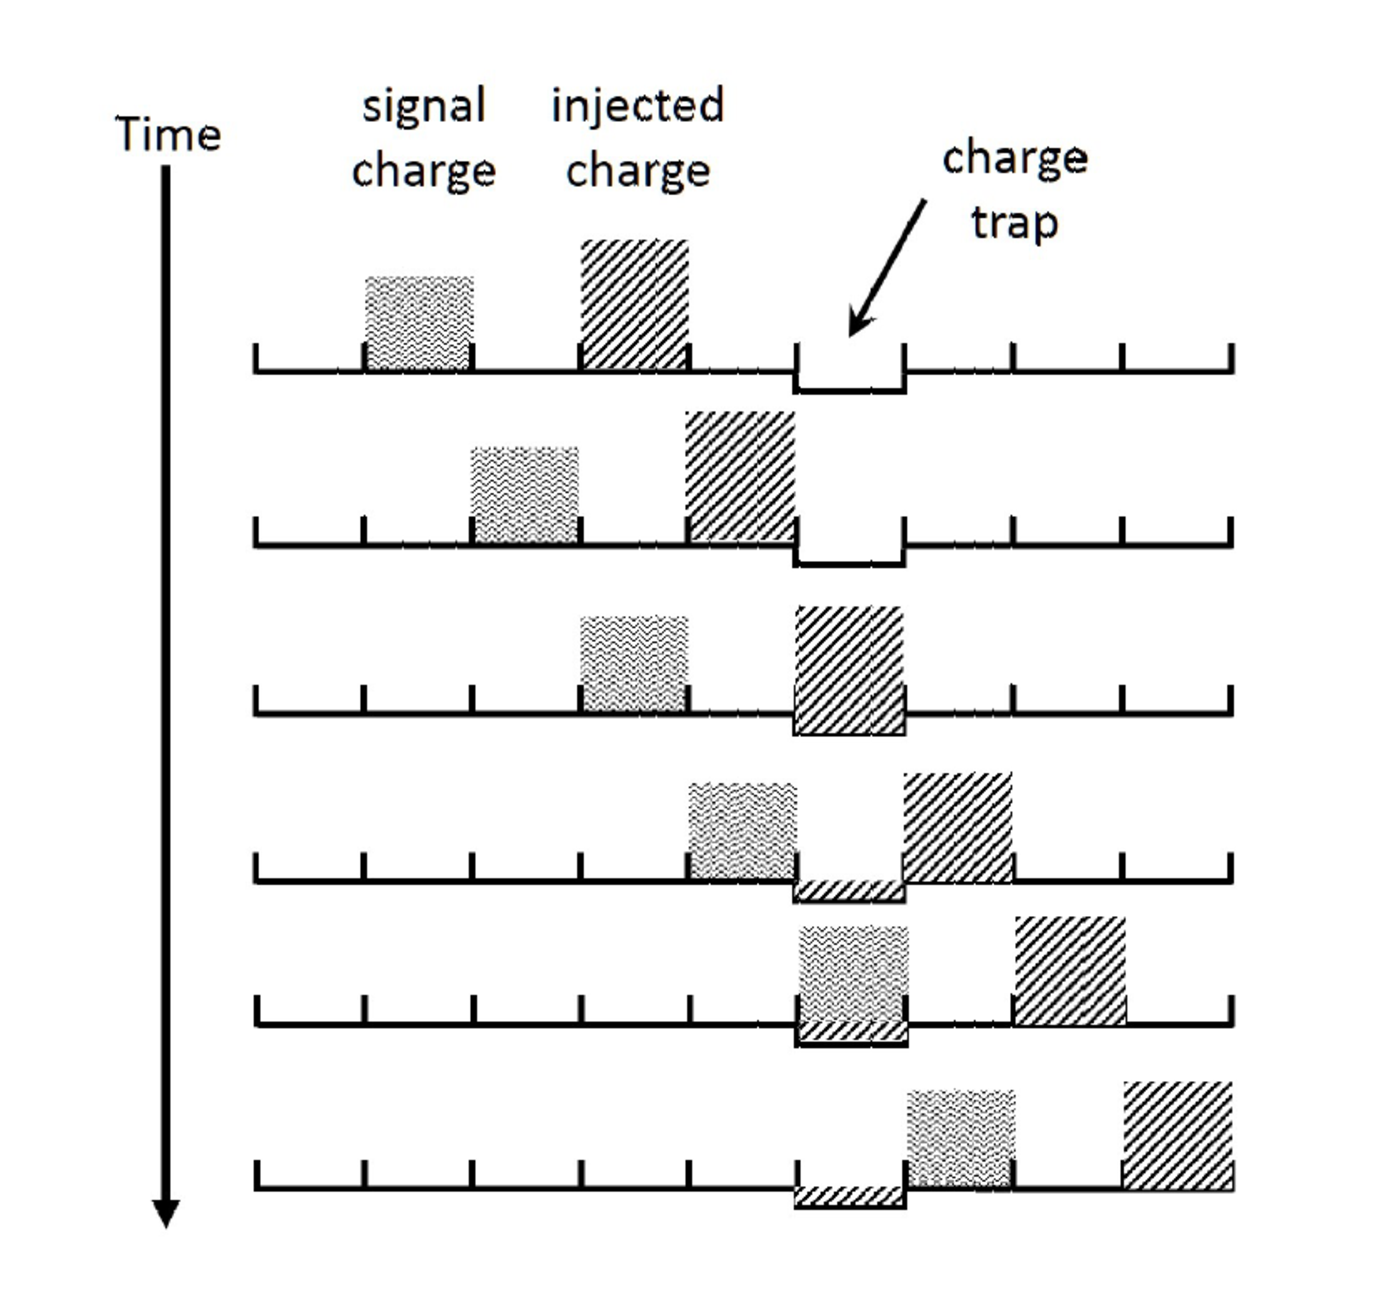
\includegraphics[width=70mm]{Chapter3/Figures/CI-kinou.eps} 
		\caption{CI を注入してトラップによる電荷損失を改善する概念図\cite{ah-jaxa}}
		\label{fig:sxi_ci_transfer}
	\end{center}
\end{figure}

\newpage
\section{静止気象衛星 GOES}

\begin{figure}[H]
	\begin{center}
		\includegraphics[width=100mm,angle=0]{Chapter3/Figures/GOES_satelite.jpg}
	\end{center}
	\caption{GOES衛星(GOES-16) の外観\cite{NOAA}。宇宙天気の観測に太陽紫外線撮像装置(SUVI)、宇宙環境現地観測装置(SEISS)、磁力計(MAG)、極端紫外線とX線放射センサー(EXIS)が使われている。太陽のX線フラックスを観測しているのが、EXISを構成しているX線センサー(XRS)である。}
	\label{fig:GOES_satelite}
\end{figure}

静止気象衛星 GOES (Geostationary Operational Environmental Satelite) は、アメリカ合衆国の静止気象衛星シリーズである。1975年に最初のGOES衛星(GOES-1)が打ち上げられ、2024年に19機目(GOES-19)が打ち上げられた。現在も運用されている GOES-16 の外観を図~\ref{fig:GOES_satelite}に示す。GOESは、地球の西半球の画像撮影や大気測定、リアルタイムの雷活動のマッピング、太陽活動と宇宙天気のモニタリングを行っている。GOESは、静止軌道(赤道上空 3万5800 km) を周回し、地球の自転と同じ速度で運行している。
GOESはアメリカ航空宇宙局(NASA)が開発と打ち上げを担当し、アメリカ海洋大気庁(NOAA)によって運用されている。

	GOES-16には以下6つの装置が搭載されている。
\begin{enumerate}
	\item Advanced Baseline Imager (ABI)
	
	\hspace{1em}地球の天気、海洋、環境を画像化する装置。ABI は、2つの可視光チャネル、4つの近赤外線チャネル、10の赤外線チャネルによって異なるスペクトルバンドで地球を観察している。
		
	\item Geostationary Lightning Mapper (GLM)
	
	\hspace{1em}雷を観測する装置。単一チャネルの近赤外線光過渡検出器で雷活動を連続的に測定している。
		
	\item Extreme Ultraviolet and X-ray Irradiance Sensors (EXIS)
	
	\hspace{1em}EXIS には、XRS と EUVS が搭載されている。XRS は太陽のX線フラックス、EUVS は太陽の極端紫外線フラックスを測定する装置。
	
	\item Magnetometer (MAG)
	
	\hspace{1em}地球周辺の磁場を測定する装置。
		
	\item Solar Ultraviolet Imager (SUVI)
	
	\hspace{1em}太陽の紫外線画像を撮影する装置。太陽のコロナや太陽フレア、コロナ質量放出などの現象を監視している。
	
	\item Space Environment In-Situ Suite (SEISS)
	
	\hspace{1em}磁気圏内のプロトン、電子、重イオンのフラックスを監視する装置。
		
\end{enumerate}
	


\subsection{X線センサー(XRS)}


\begin{figure}[H]
	\begin{center}
		\includegraphics[width=100mm,angle=0]{Chapter3/Figures/GOES_XRS.jpg}
	\end{center}
	\caption{GOESのX線センサー(XRS)の断面図。(Thomas et al.2024)\cite{Thomas}}
	\label{fig:GOES_XRS_view}
\end{figure}

図~\ref{fig:GOES_XRS_view}にGOES /XRS の断面図を示す。光学キャビティの外側は、軽い元素でできたアルミニウム(Al)のハウジング(緑)で覆われており、内側の壁は重い元素を含む銅タングステン合金(オレンジ)で作られている。さらに、X線を制御するベリリウム(Be)フィルターや、光を検出するフォトダイオード、測定データを処理する電子回路、視野を調整するバッフルやコリメーター、磁気を利用したアセンブリ(灰色)も含まれている。

表~\ref{tb:GOES_XRS_perform}にGOES /XRS の主な性能を示す。 GOES には2台の XRS が搭載されており、XRS-A では、0.09-0.37 nm、XRS-B では、0.10-0.69nm の波長帯の太陽X線フラックスを観測している。XRS-B で観測された 0.10-0.69 nm(1-8\AA) のエネルギー帯で測定されたX線フラックスをもとに、太陽フレアの等級分けがされる。$ 10^{-8}$ $\mathrm{W/m^2} $ レベルをAクラスとし、一桁ずつX線フラックスが上がるごとに, B, C, M, Xクラスとクラス分けされている。また, X線フラックスの値との対応をとるために、$5.0^{-6}$ $\mathrm{W/m^2} $ のときには、C5.0 クラスと表記される。表~\ref{tb:GOES_XRS_perform}に示す帯域外除去率とは、指定されたスペクトル範囲外の信号をどの程度抑制できるかを示す指標である。放射照度範囲とは、センサーが検出可能な放射照度の範囲である。分解能(3-s,$ \mathrm{W}/\mathrm{m}^2 $)とは、3秒間の平均値として測定される最小の放射照度変化量を示している。数値が小さいほど、微細な変化を検出できる高い分解能を持つことを意味する。精度(3-s,$ \mathrm{W}/\mathrm{m}^2 $)とは、3秒間の平均値として測定される放射照度の測定精度である。放射照度の正確さは、測定された放射照度値が実際の値とどの程度一致しているかを示す指標である。視野角は、センサーの視野角を分単位で示した値である。

\begin{table}[htbp]
	\begin{center}
		\caption{XRSの主な性能(Thomas et al.2024)\cite{Thomas}}
		\label{tb:GOES_XRS_perform}
		\begin{tabular}{ccccc}
			\hline \hline
			パラメータ & XRS-A channel & XRS-B channel\\ \hline
			スペクトル範囲(nm) & 0.09-0.37 & 0.10-0.69  \\
			帯域外除去率(\%) & 2.8\% & 6.3\%  \\
			放射照度範囲($ \mathrm{W}/\mathrm{m}^2 $) & $10^{-9}$ to $10^{-2}$ &  $10^{-9}$ to $10^{-2}$ \\
			分解能(3-s,$ \mathrm{W}/\mathrm{m}^2 $) & $3.0 \times 10^{-10}$ &  $2.5 \times 10^{-10}$ \\			
			精度(3-s,$ \mathrm{W}/\mathrm{m}^2 $) & $3.8 \times 10^{-9}$ & $3.8 \times 10^{-9}$ \\	
			放射照度の正確さ(\%) & 10\% &  10\%\\
			視野角(FOV, arcmin) & $ \pm 70 $ & $ \pm 70 $	
			\\\hline
		\end{tabular}
	\end{center}
\end{table}